\documentclass{article}
\usepackage{graphicx} %package to manage images
\usepackage[utf8]{inputenc}
\usepackage[a4paper, total={6in, 8in}]{geometry}
\usepackage{xurl}
\title{Relatório 4 \\ Pré-processamento}
\author{Pedro A. S. O. Neto}
\date{Fevereiro 2022}

\begin{document}

\maketitle

\section{Verificando consistência dos dados}

\subsection{Problema 1} 
O máximo tempo de fixação reportado nos dados é de 8ms. Precisamos mudar os parâmetros de extração dos dados para que fixações sejam agrupadas em tempos maiores. Nessas análises, eu escrevi um código para agrupar essas fixações, mas o ideal seria trabalhar com o dado inalterado do Tobii.

\subsection{Problema 2}
Existem 2 aplicações da mesma trial na mesma timeline. No entanto, Não existe indicação, nos dados, de quando termina uma trial e começa a outra. Um exemplo da consequência  dessa falha está na figura abaixo, no trial (RJA.A2.B2.E, RJA.A1.B2.D).

\section{Primeira visualização dos dados}

Os códigos foram desenvolvidos para um subconjunto dos dados totais. O eixo x indica tempo, e o eixo y indica o objecto (Rosto, Brinquedo Esquerda e Brinquedo Direita). Em cada trial, a última letra indica qual brinquedo a criança deve olhar. E: Esquerda; D: Direita.

Os gráficos abaixo estão separados por criança. Seria interessante verificar se as informações dos gráficos coincidem com os vídeos das crianças. Isso é uma forma de validação externa das minhas análises/processamento dos dados. Enquanto não acertarmos o \textbf{Problema 2}, ignorem os trials com grandes períodos vazios entre fixações. Eles indicam as trials que foram aplicadas duas vezes.

\begin{figure}[t]
\caption{Abacaxi}
\noindent\makebox[\textwidth]{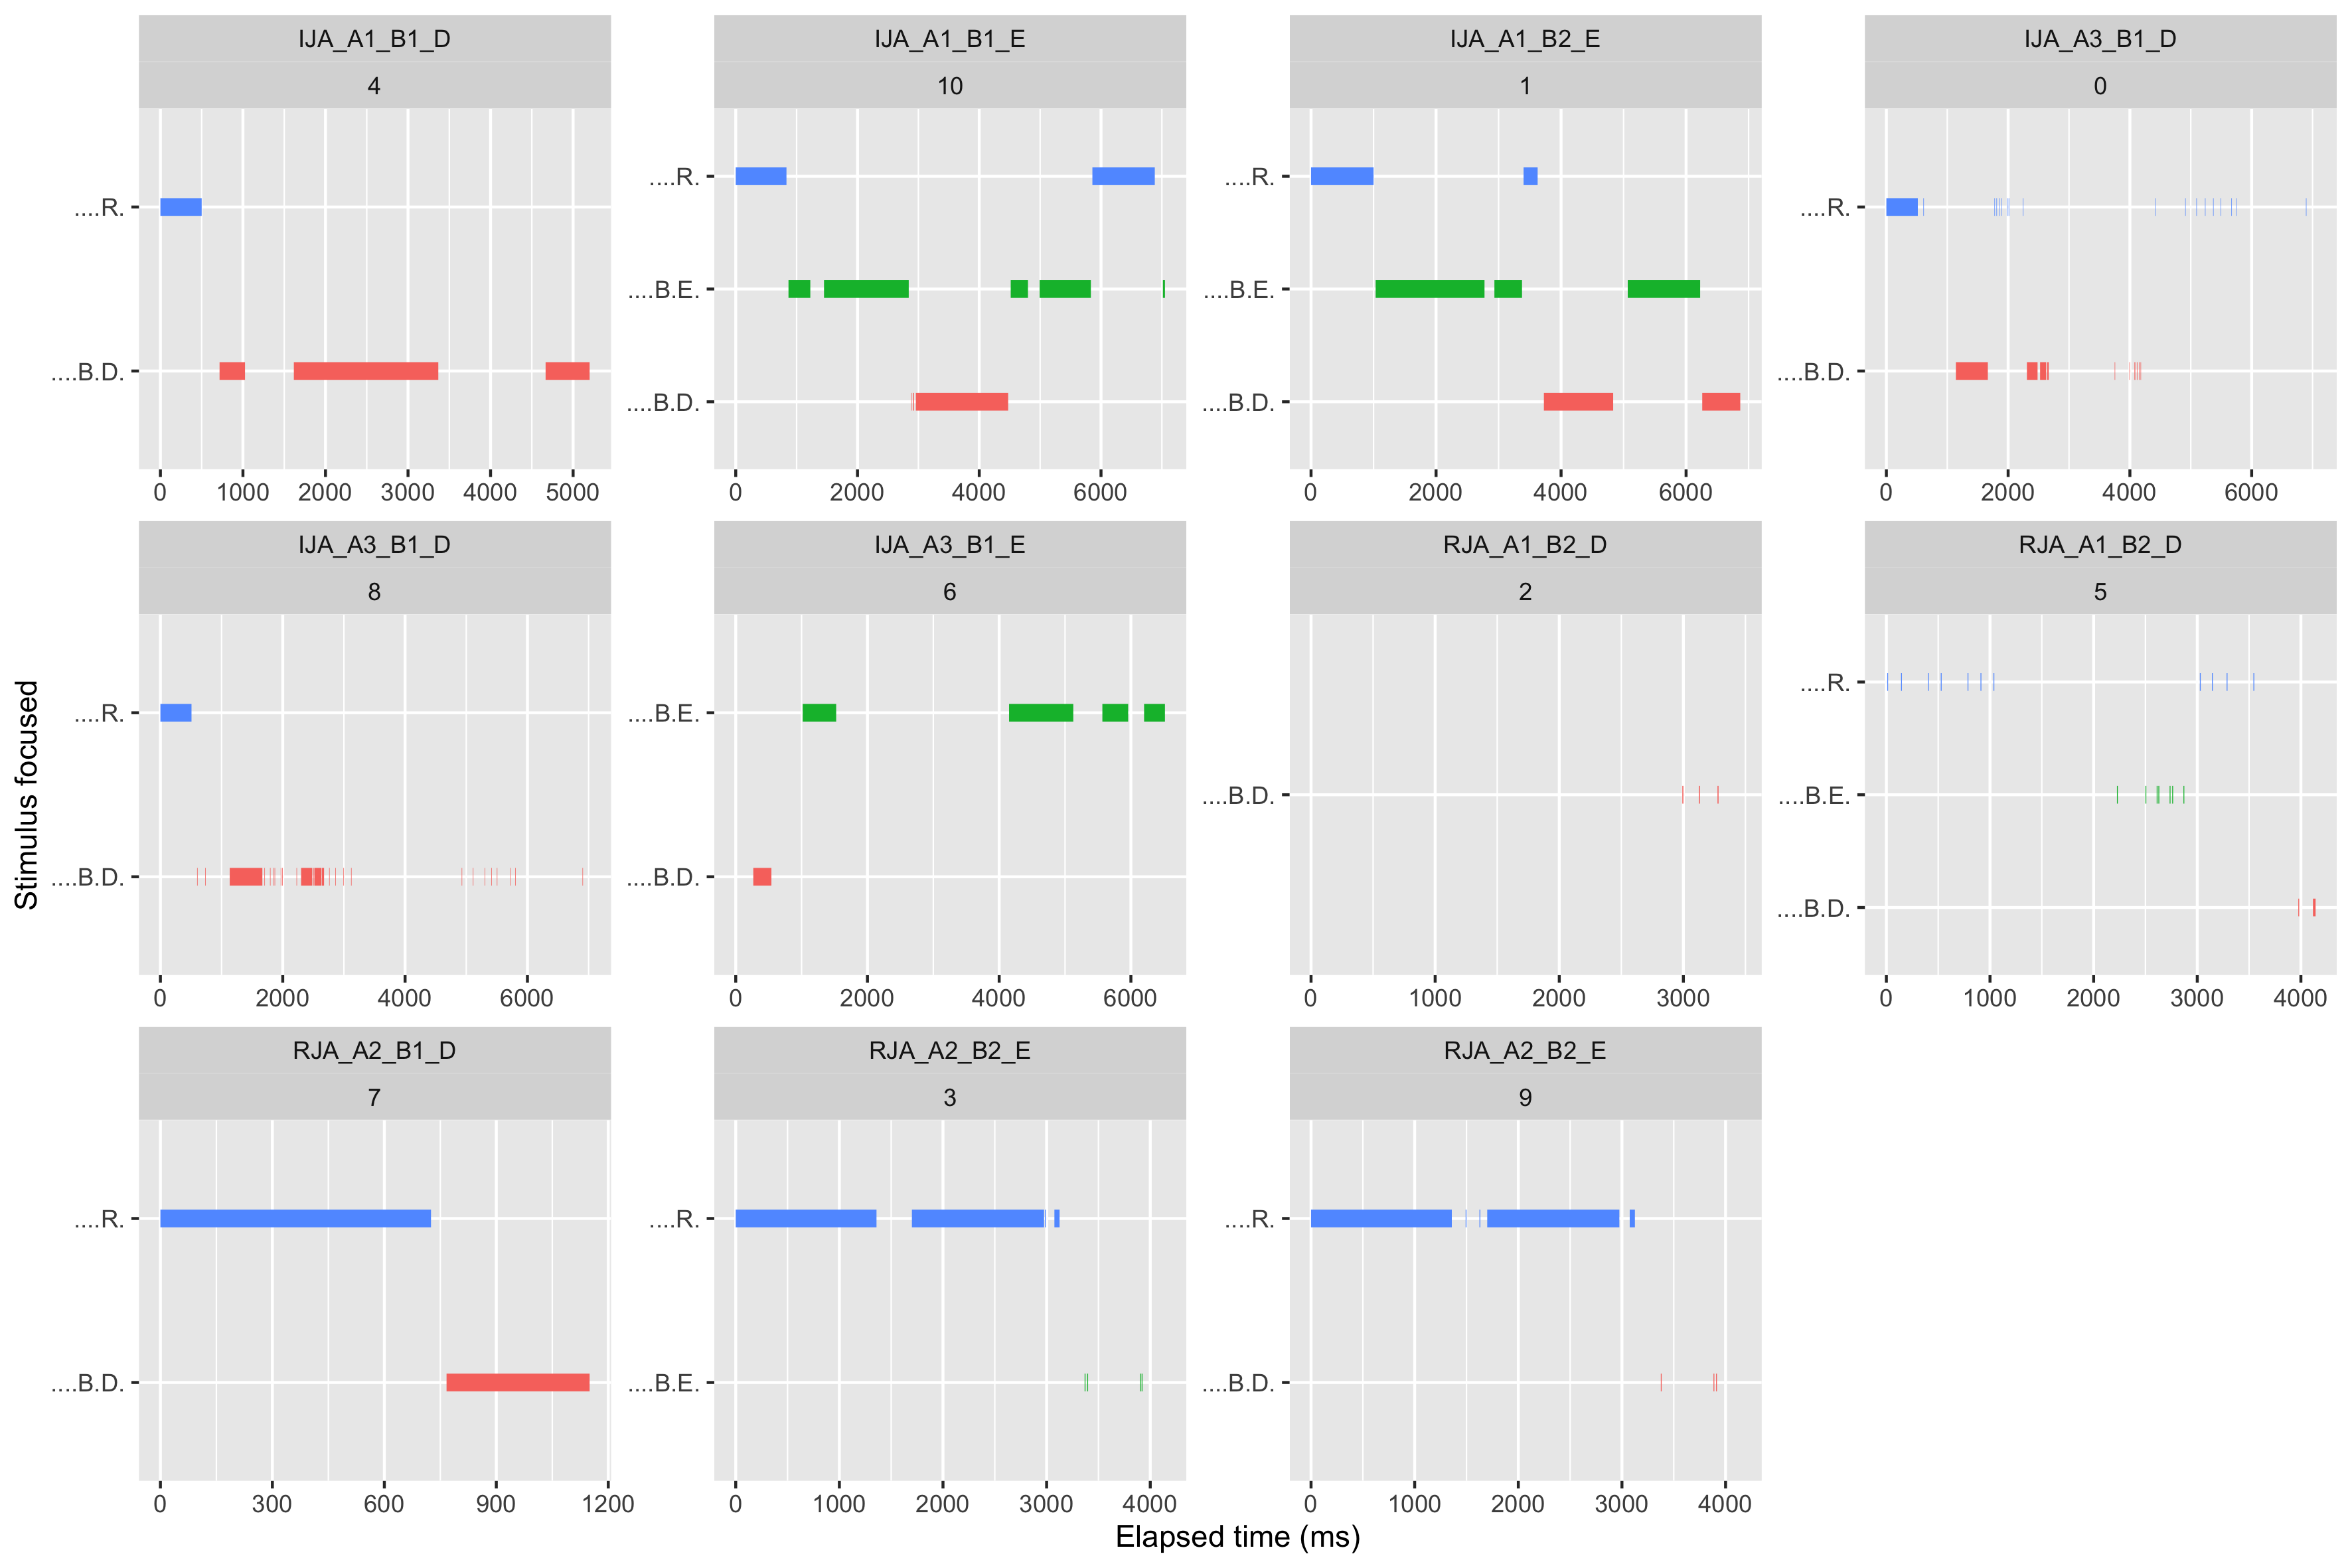
\includegraphics[width=\paperwidth]{"./graph_visu1.png"}}
\centering
\end{figure}

\begin{figure}[t]
\caption{Babacu}
\noindent\makebox[\textwidth]{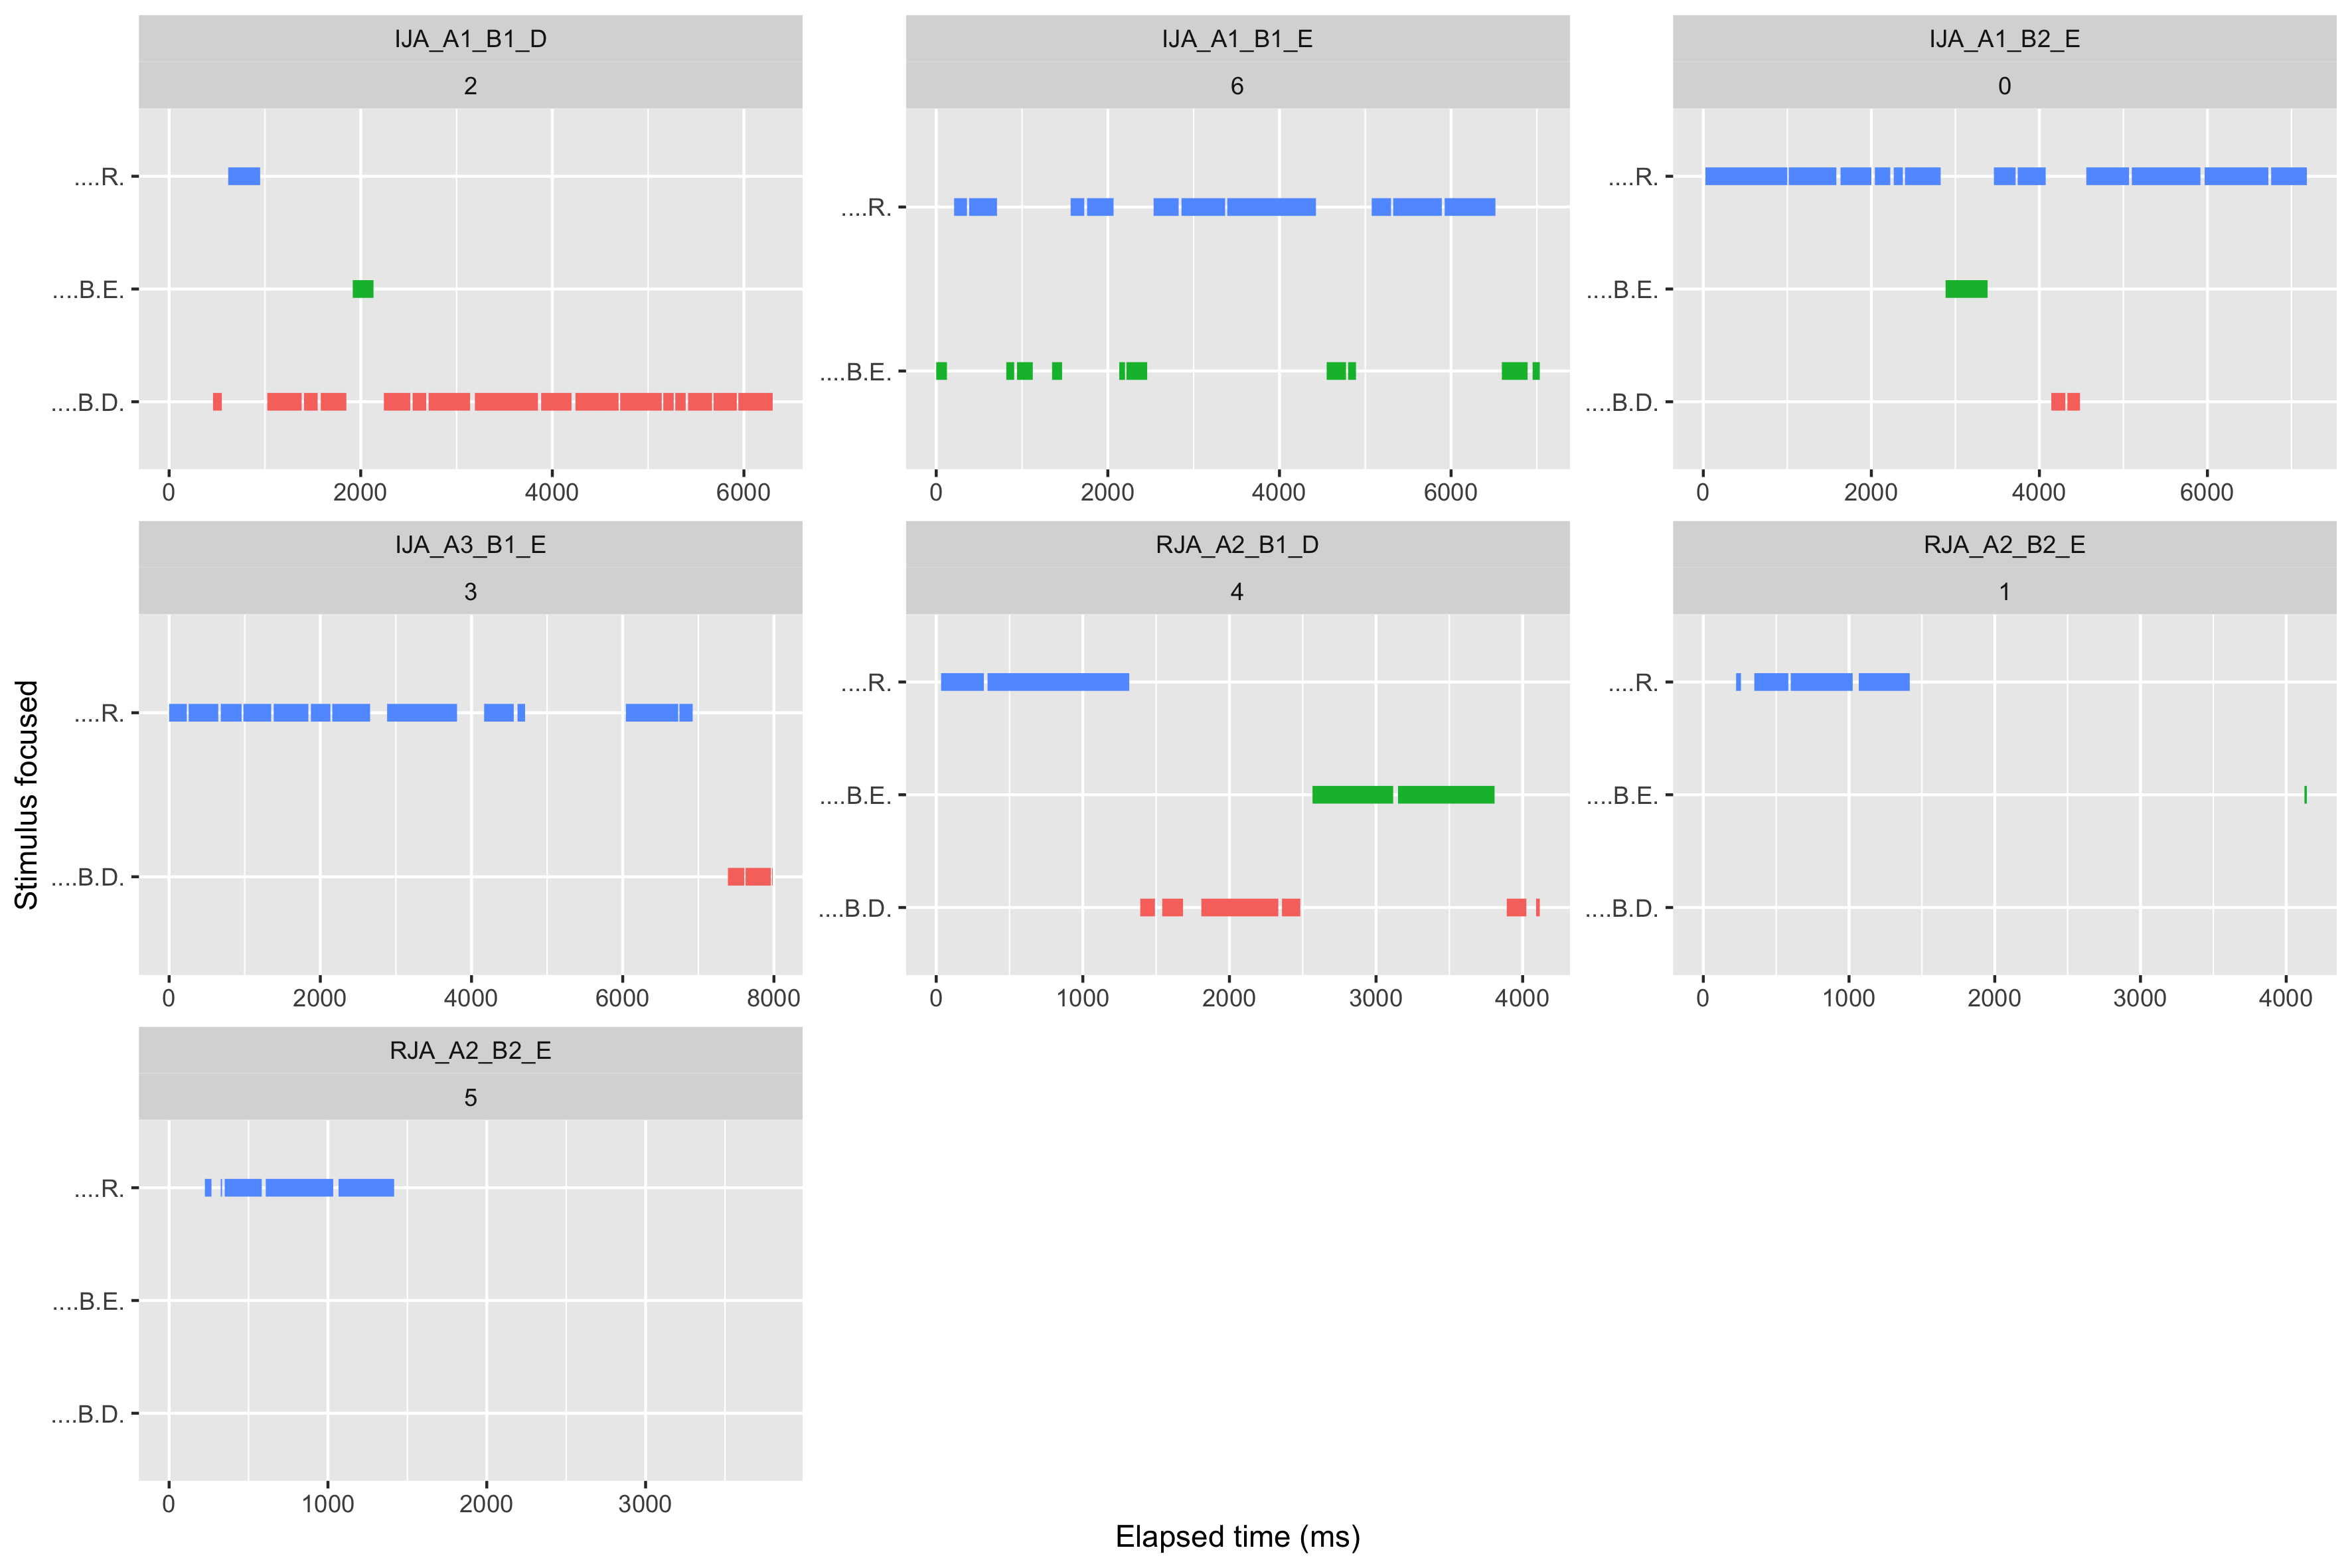
\includegraphics[width=\paperwidth]{"./graph_visu2.png"}}
\centering
\end{figure}

\begin{figure}[t]
\caption{Baru}
\noindent\makebox[\textwidth]{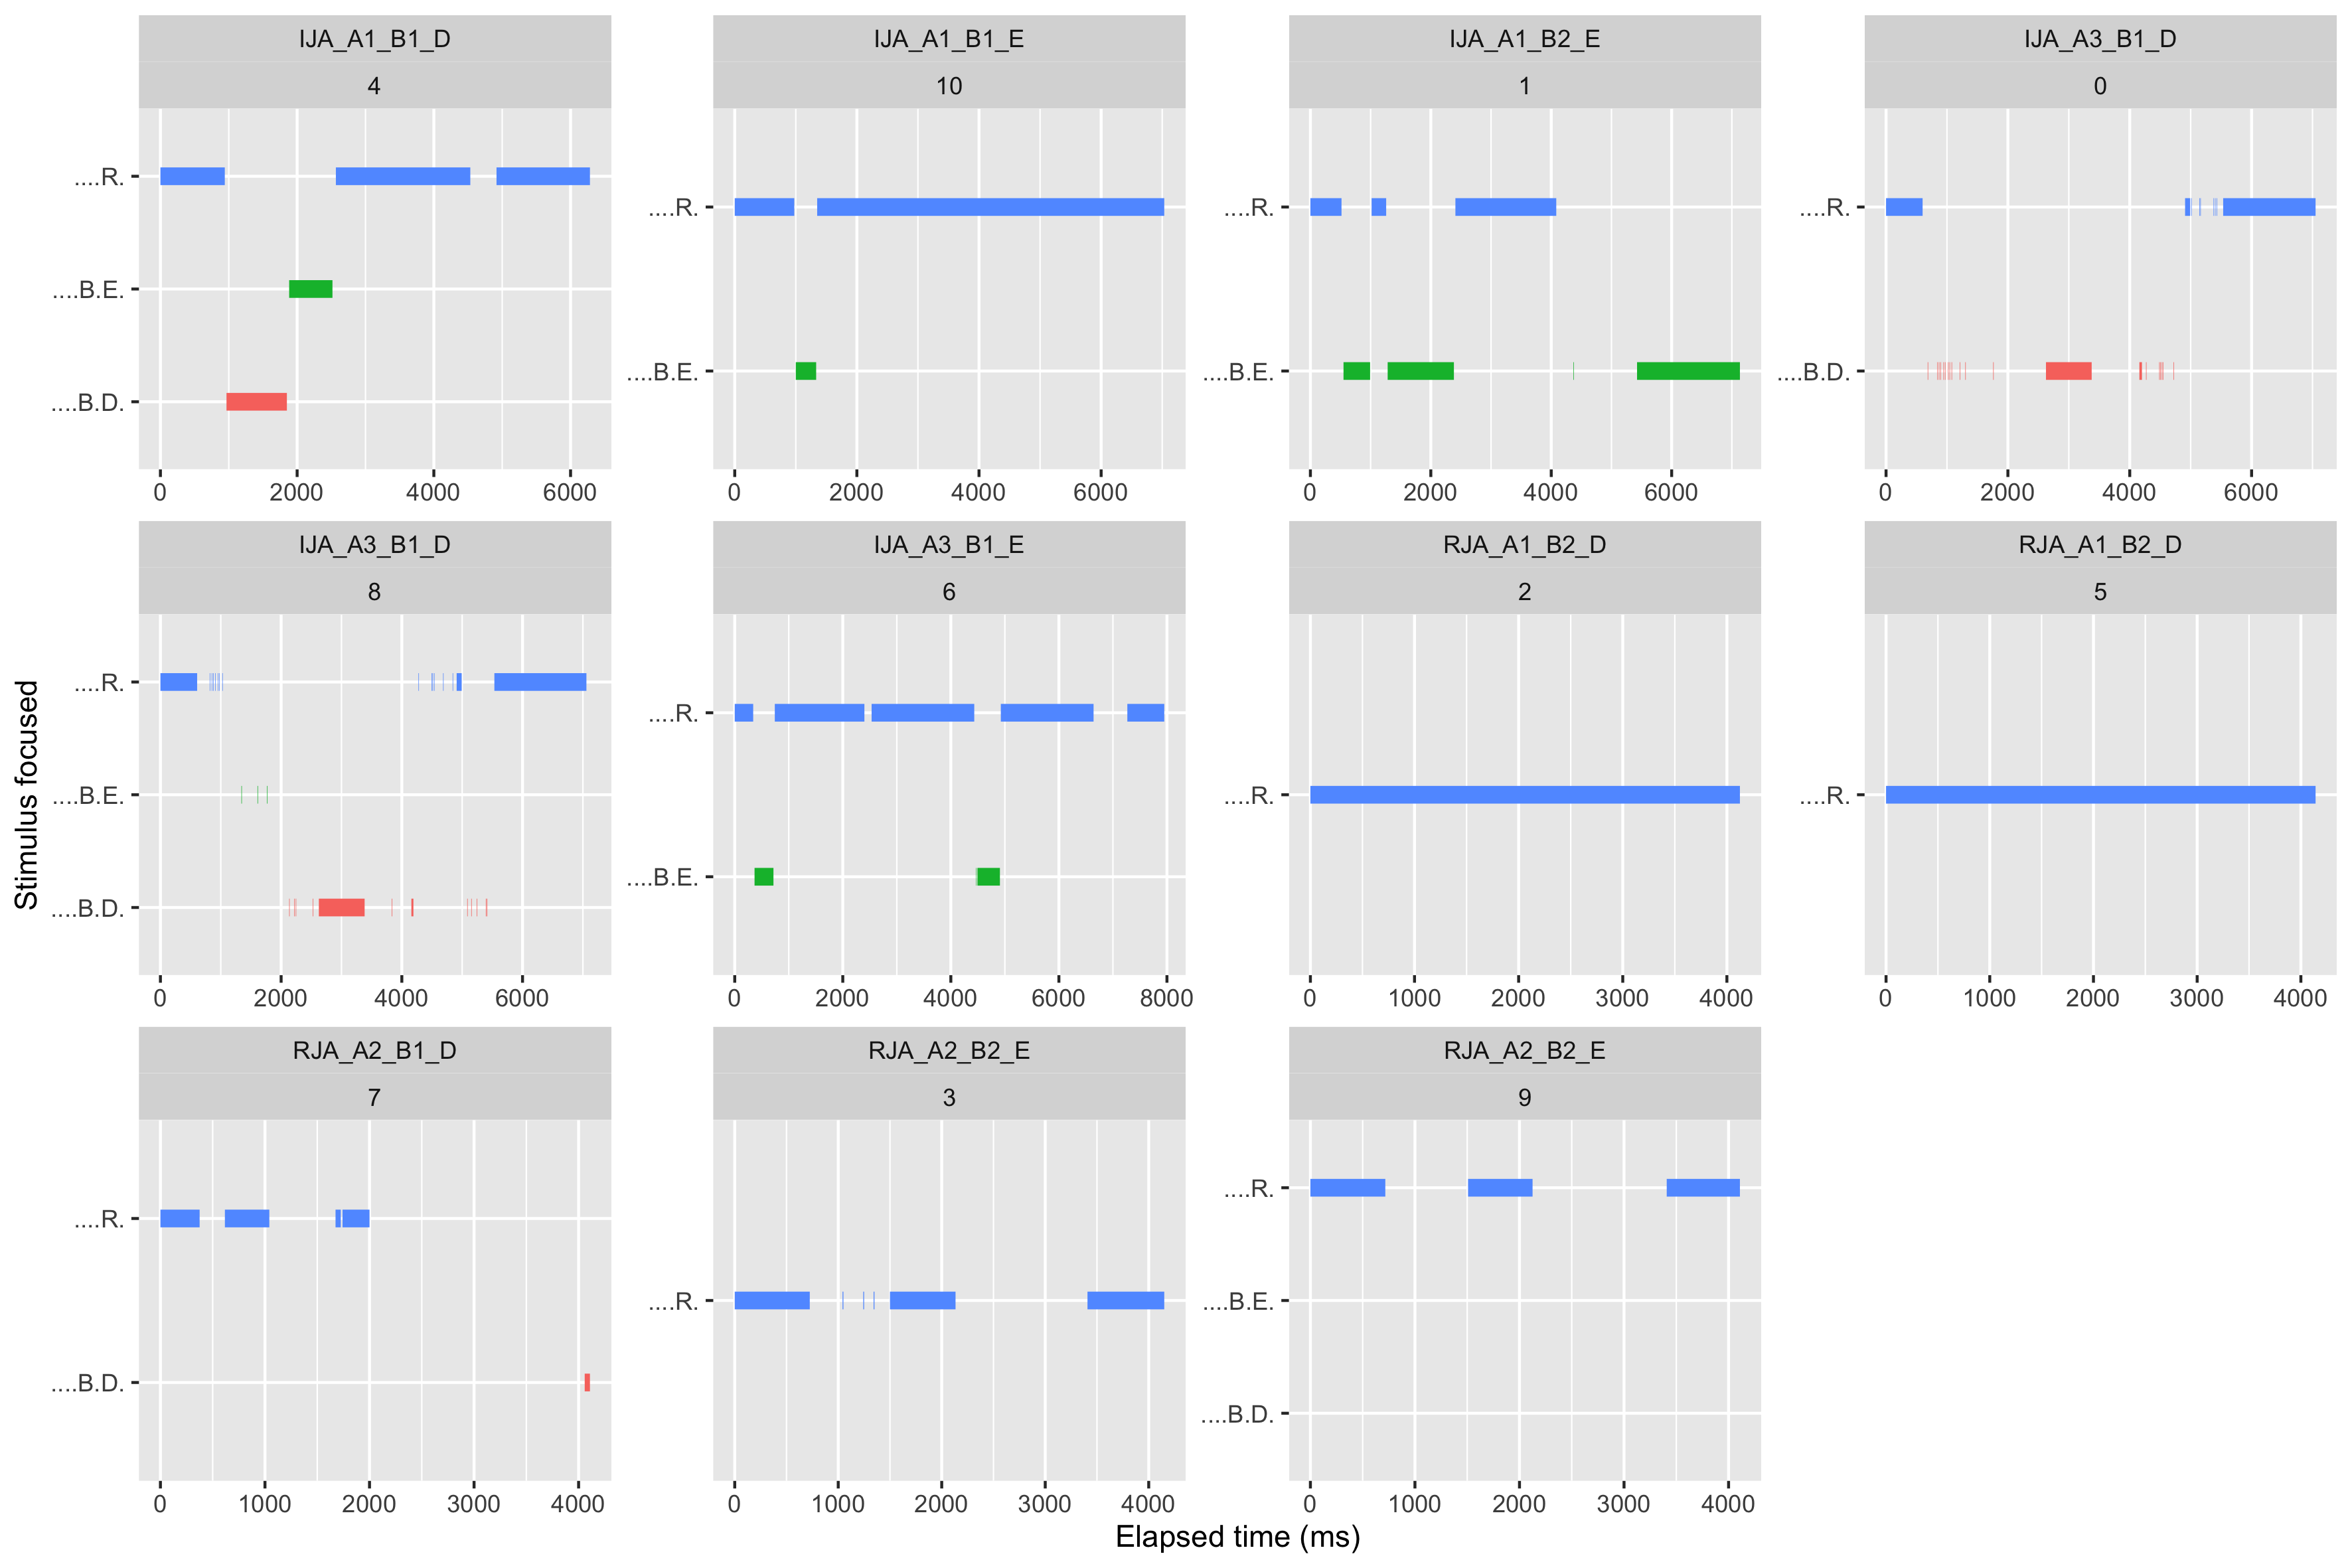
\includegraphics[width=\paperwidth]{"./graph_visu3.png"}}
\centering
\end{figure}

\begin{figure}[t]
\caption{Dovyalis}
\noindent\makebox[\textwidth]{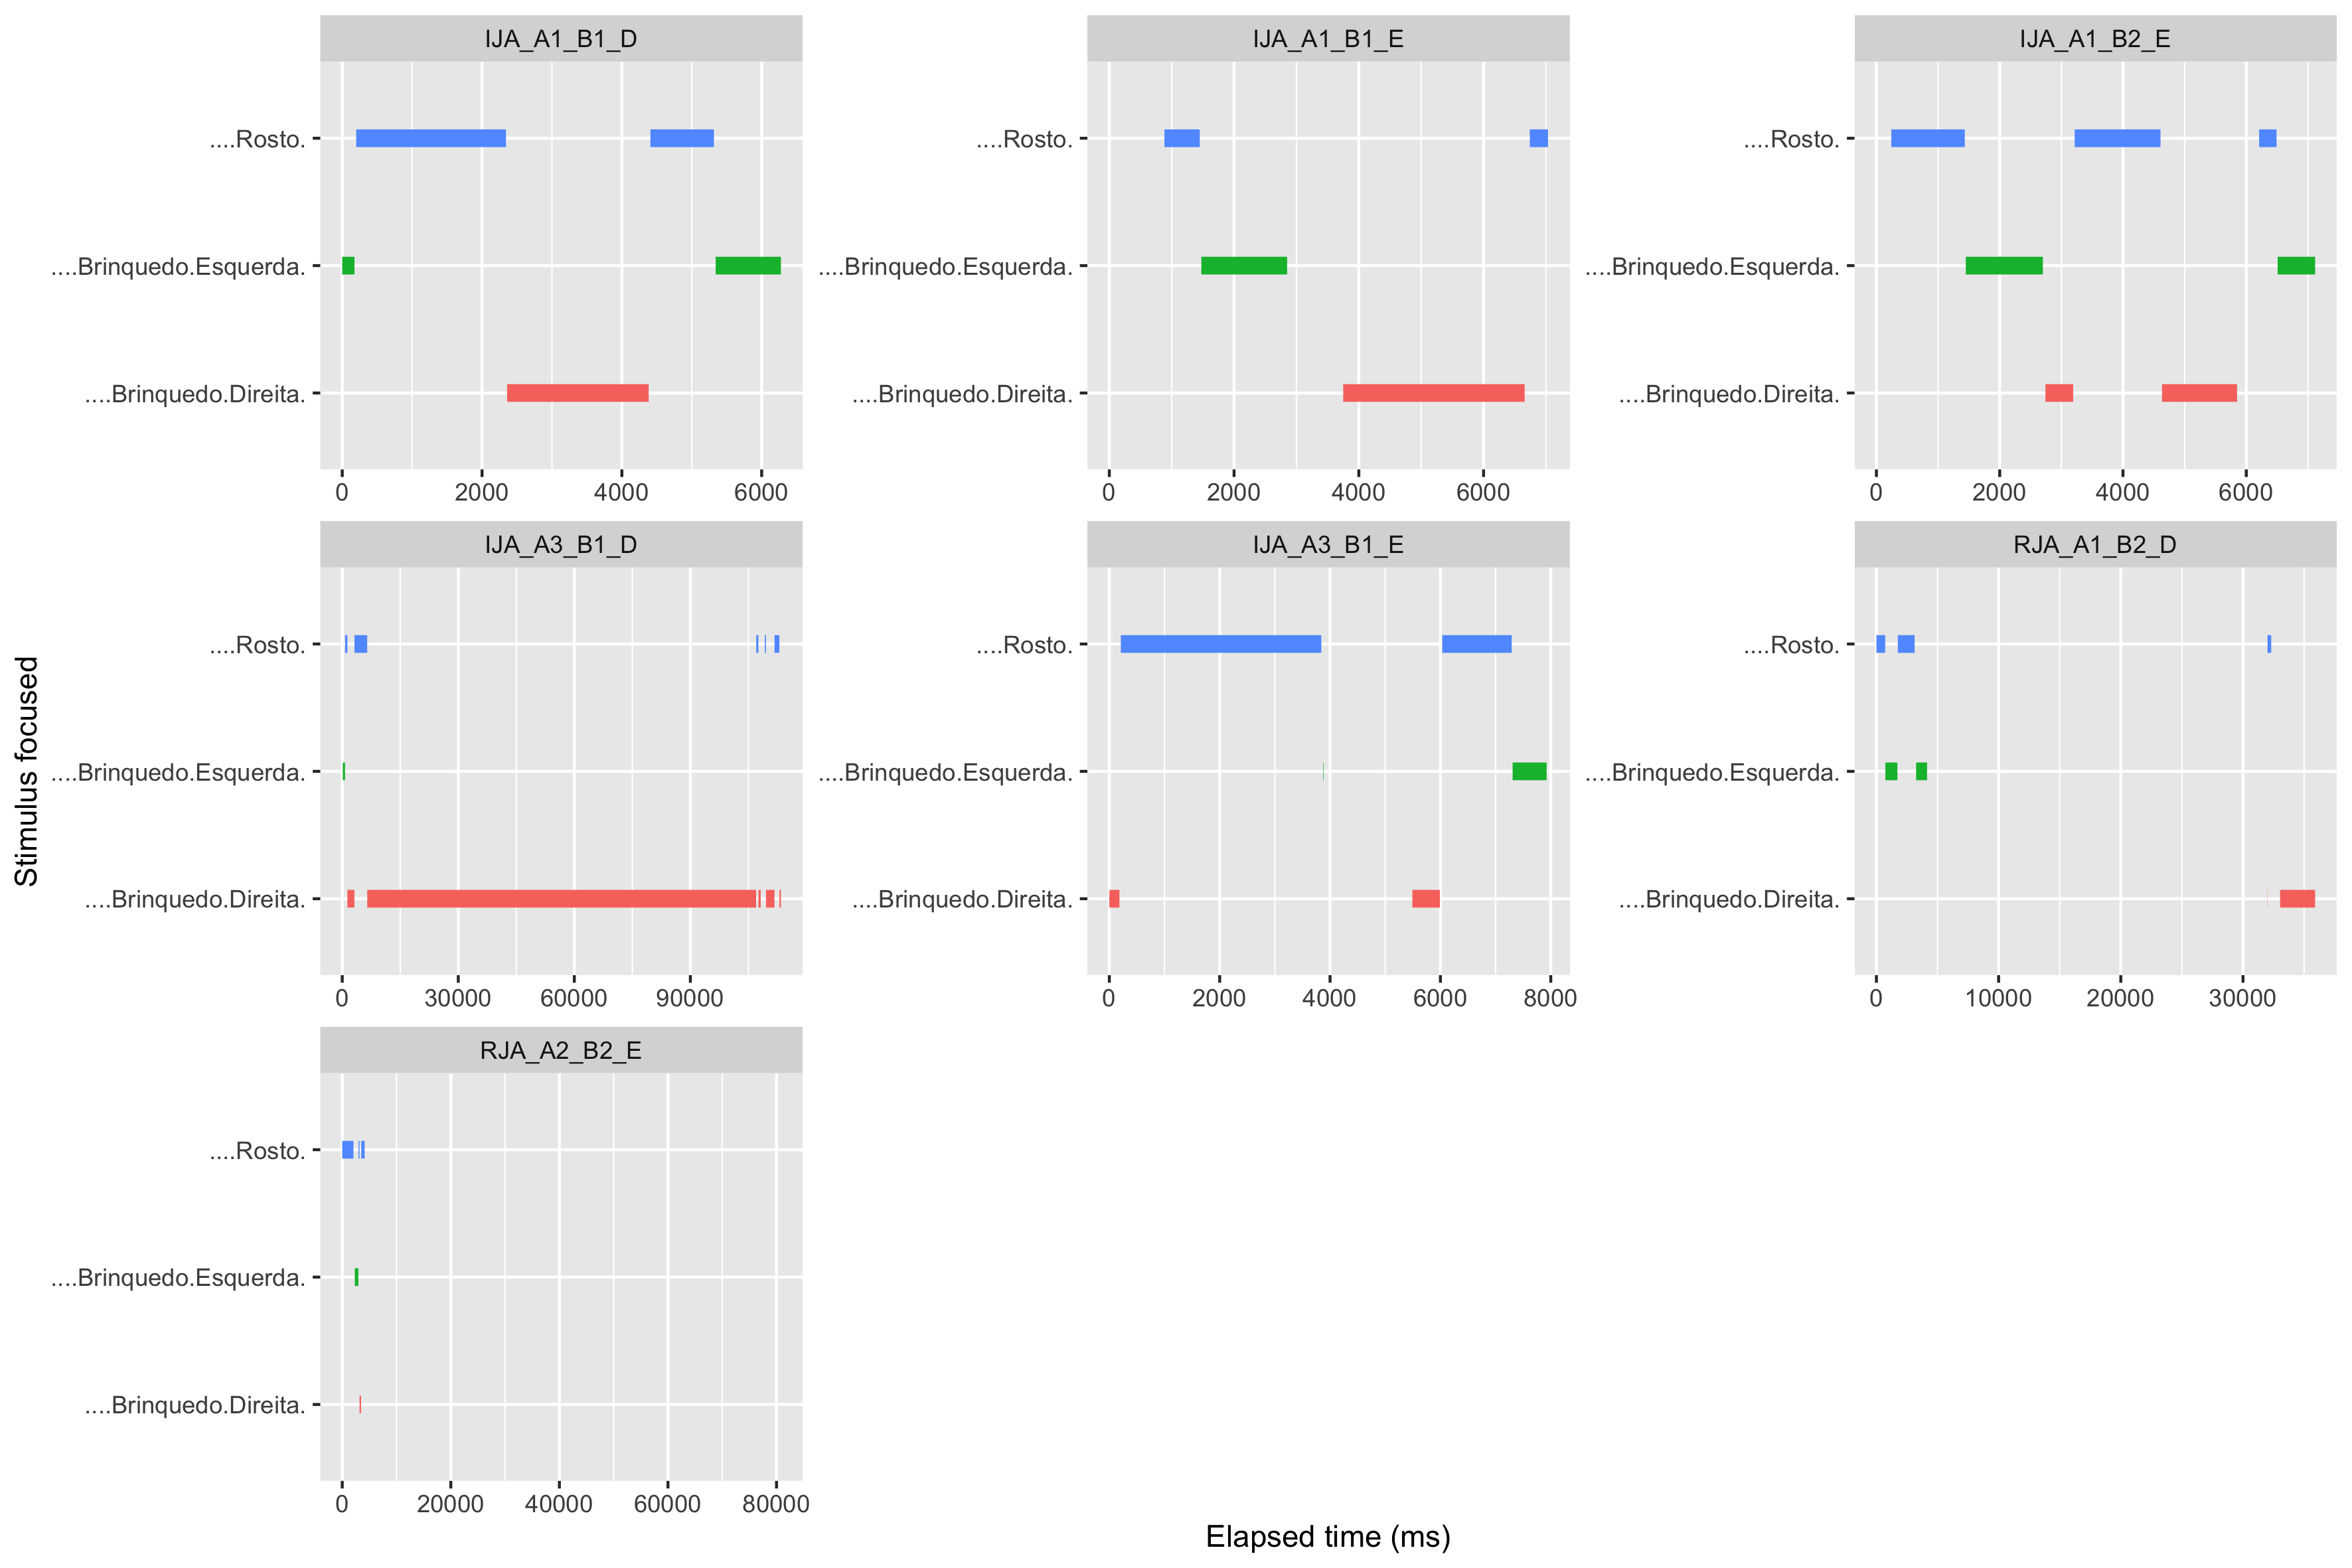
\includegraphics[width=\paperwidth]{"./graph_visu4.png"}}
\centering
\end{figure}

\begin{figure}[t]
\caption{Safira}
\noindent\makebox[\textwidth]{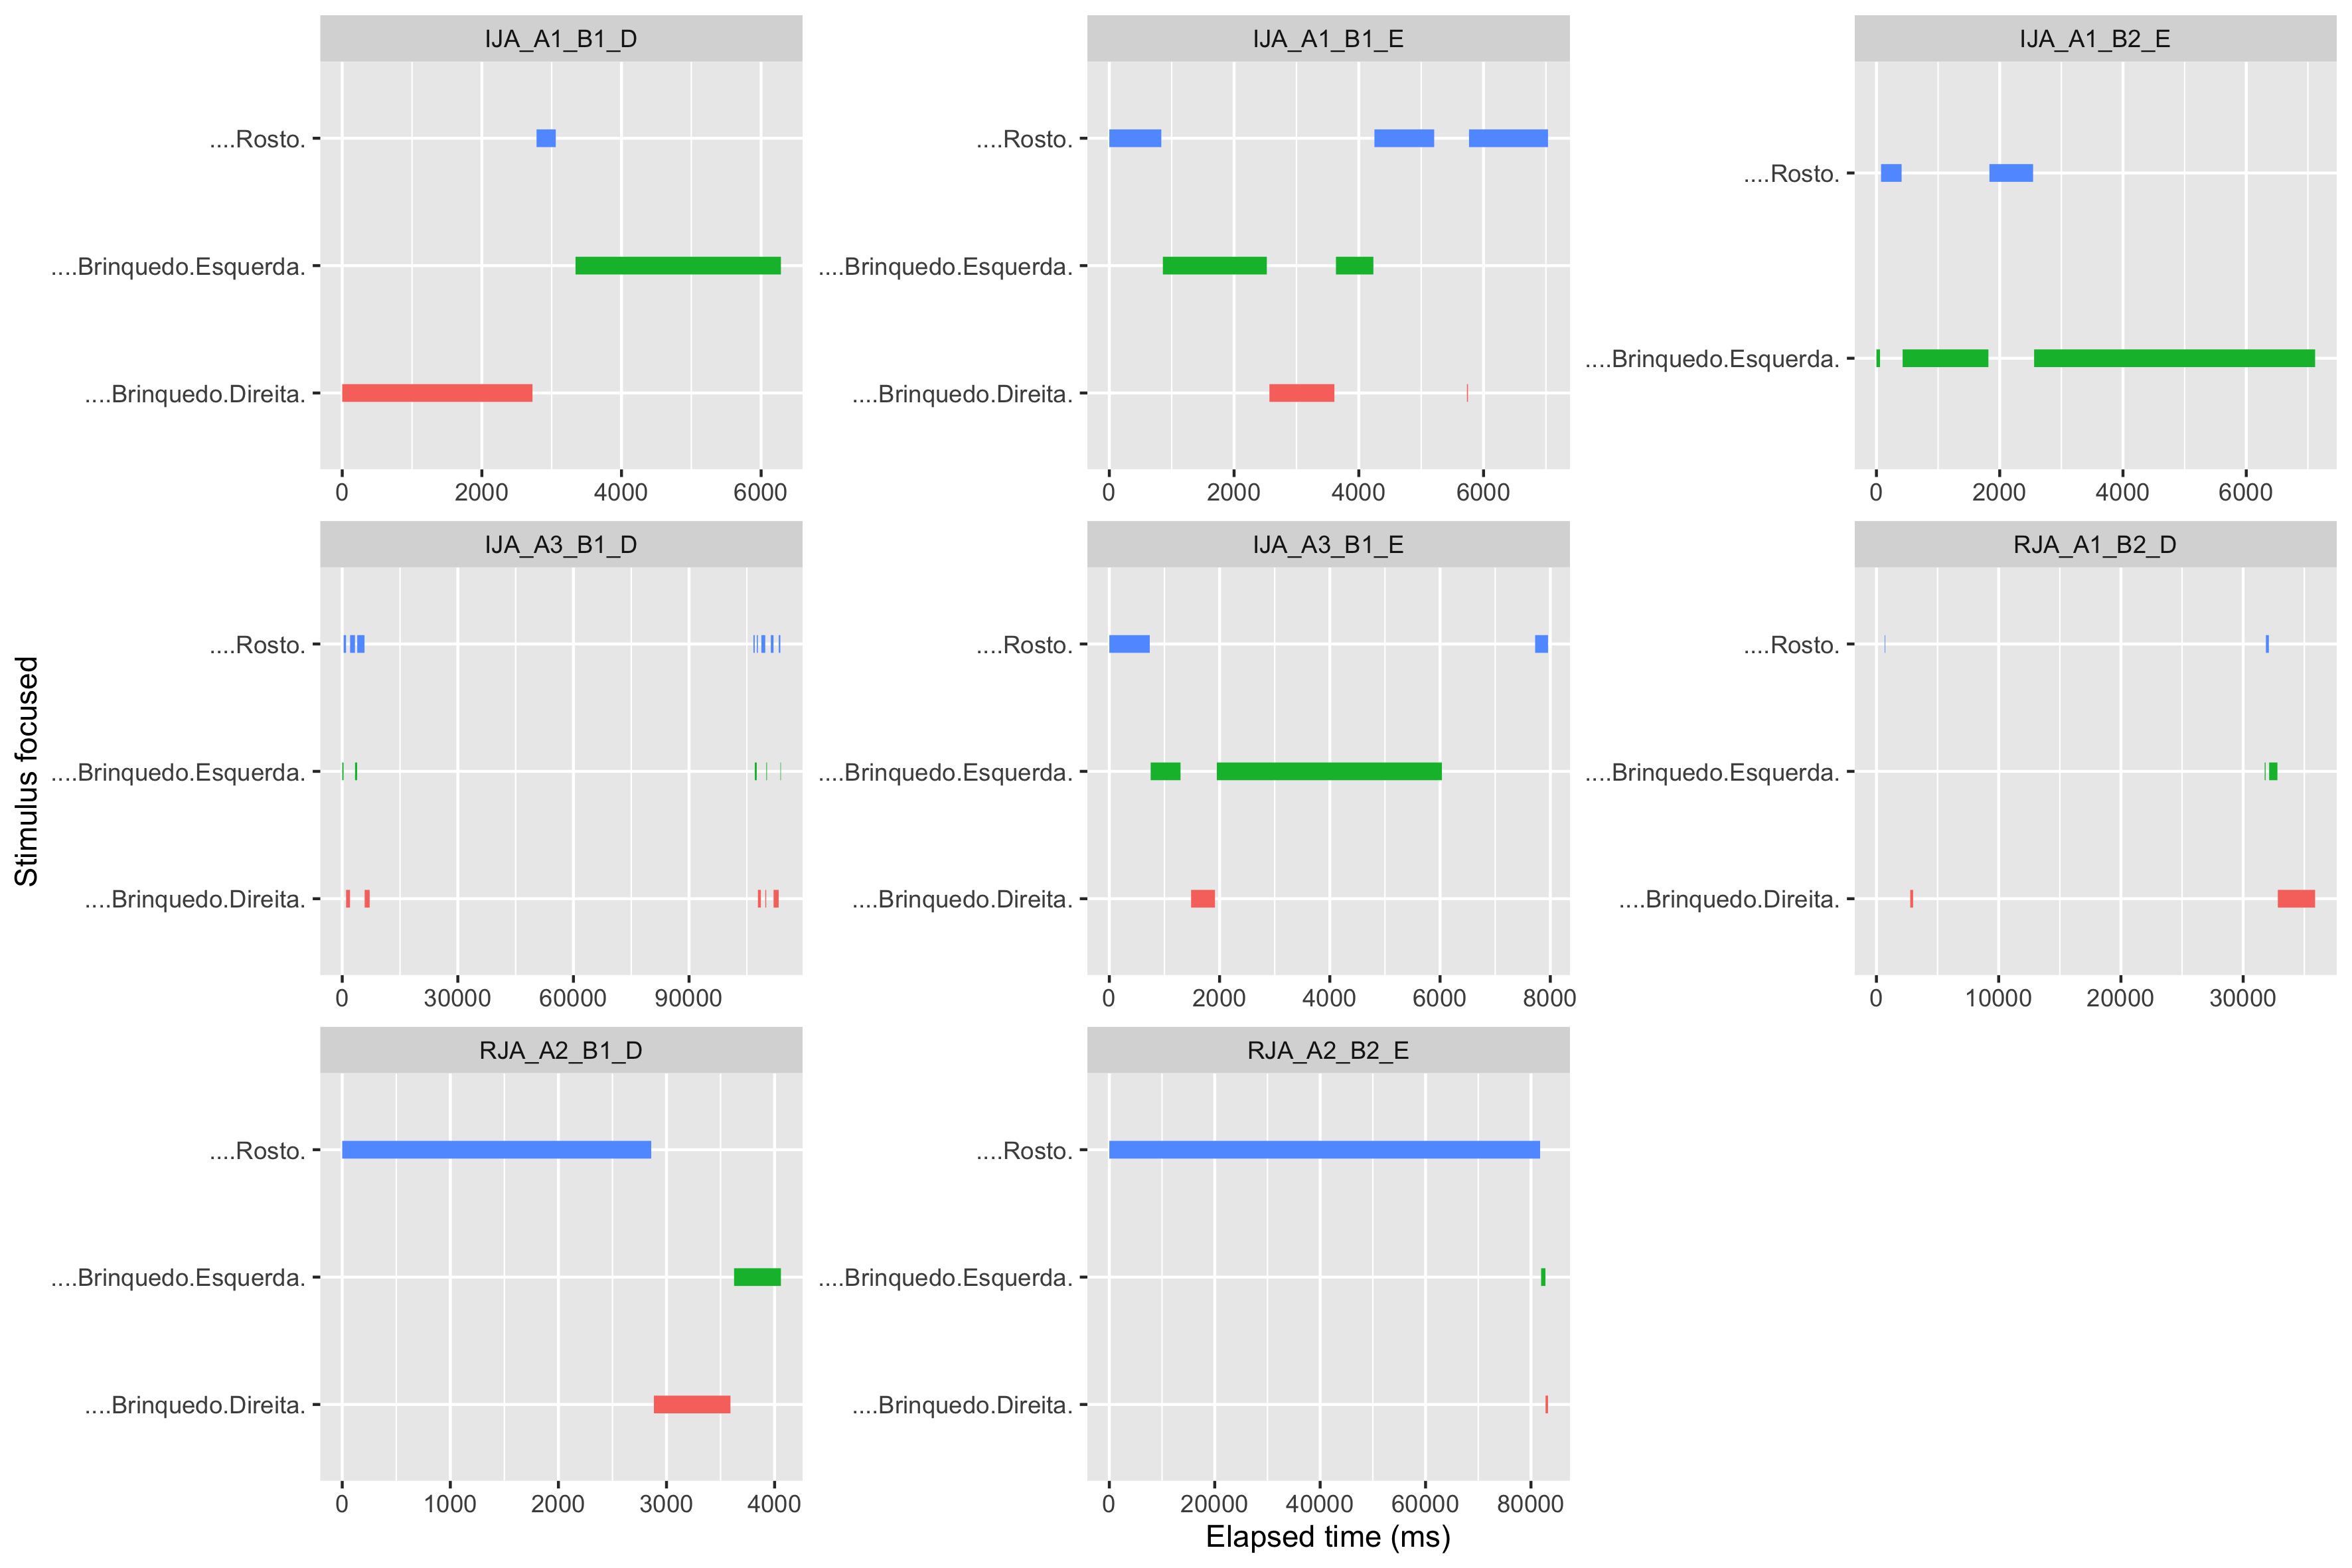
\includegraphics[width=\paperwidth]{"./graph_visu5.png"}}
\centering
\end{figure}

\end{document}


